\documentclass{book}

\usepackage{graphicx,epsfig}
\usepackage{hyperref}
\usepackage{amsmath,amssymb}
\usepackage{array}
\usepackage[toc,page]{appendix}

\graphicspath{{figures/}}

\renewcommand{\baselinestretch}{1}

\setlength{\textheight}{9in}
\setlength{\textwidth}{6.5in}
\setlength{\headheight}{0in}
\setlength{\headsep}{0in}
\setlength{\topmargin}{0in}
\setlength{\oddsidemargin}{0in}
\setlength{\evensidemargin}{0in}
\setlength{\parindent}{.3in}
\pagestyle{plain}

\begin{document}
\bibliographystyle{plain}

\large

% ============================================================ TITLE PAGE
\thispagestyle{empty}
\centerline{\bf A REPORT}
\vspace*{0.3cm}
\centerline{\bf ON}
\vspace*{0.3cm}
\centerline{\bf NEURO-SYMBOLIC GENERATION AND FORMAL}
\vspace*{0.15cm}
\centerline{\bf VERIFICATION OF ARCHITECTURAL FLOOR PLANS}
\vspace*{2cm}

\centerline{BY}
\vspace*{1cm}

\begin{center}
	\begin{tabular}{lll}
		Name of the student & \hspace*{2cm} ID No. & \hspace*{2cm} Discipline \\
		Ojas Marathe &\hspace*{2cm} 2024A7PS0645G &\hspace*{2cm} B.E. in Computer Science \\ % FILL: ID and discipline
	\end{tabular}
\end{center}

\vspace*{2cm}
\begin{center}
	{\bf Prepared in partial fulfillment of the \\
	Practice School - II Course} \\
\end{center}

\vspace*{0.5cm}
\centerline{AT}
\vspace*{1cm}
\centerline{\bf AI Gurukul} % FILL: confirm exact station name
\vspace{0.2cm}
\centerline{\bf A Practice School - II}
\vspace{0.2cm}
\centerline{\bf Station of}
\vspace{0.5cm}

% Add your BITS Pilani logo below (logo.pdf or logo.png) and uncomment:
% \begin{figure}[ht]
% \centerline{\includegraphics[width=1.0in]{logo}}
% \end{figure}
\vspace{1cm}

\centerline{\bf BIRLA INSTITUTE OF TECHNOLOGY \& SCIENCE, PILANI}
\vspace*{0.5cm}
\centerline{\bf June, 2026}
\newpage

% ============================================================ PS DIVISION PAGE
\thispagestyle{empty}
\centerline{\bf BIRLA INSTITUTE OF TECHNOLOGY \& SCIENCE, PILANI}
\vspace*{0.2cm}
\centerline{\bf Practice School Division}
\vspace*{0.3cm}
{\bf
	\begin{tabular}{p{6cm}l}
		& \\ & \\ & \\
		Station: AI Gurukul & \hspace*{2cm} Centre: Online \\ % FILL
		& \\
		Duration: 8 weeks &\hspace*{2cm} Date of start: 26/05/2026 \\ % FILL
		& \\
		Date of submission: 20/06/2026 & {} \\
		& \\
		Title of the project: & \\
		\multicolumn{2}{p{14cm}}{Neuro-Symbolic Generation and Formal Verification of Architectural Floor Plans} \\
		& \\
		ID No., Name and Discipline of the student: & \\
		\multicolumn{2}{p{14cm}}{2024A7PS0645G, Ojas Marathe, B.E. in Computer Science} \\ % FILL
		& \\
		Name and Designation of the expert: & \\
		\multicolumn{2}{p{14cm}}{Anupam Purwar, Mentor} \\ % FILL
		& \\
		Name of the PS faculty member: & \\
		\multicolumn{2}{p{14cm}}{Muhammed Sajid N} \\ % FILL
		& \\
		Key words: & \\
		\multicolumn{2}{p{14cm}}{Neuro-symbolic AI; SMT (Z3); Mixed-Integer Linear Programming; Large Language Models; Computer-Aided Design; Building-code verification; Human-in-the-loop} \\
		& \\
		Project areas: & \\
		\multicolumn{2}{p{14cm}}{Agentic AI, Automated CAD, Formal Verification} \\
		& \\
		Abstract: & \\
		\multicolumn{2}{p{14cm}}{This project builds a two-agent, neuro-symbolic system that generates and \emph{formally verifies} architectural drawings of a single-family house. A Large Language Model (and, alternatively, a Mixed-Integer Linear Programming solver) proposes the geometry of the house's outer boundary and its interior room layout, while the Z3 SMT solver acts as a deterministic judge that checks every Seattle Building Code and IRC constraint. Generated code is never executed: geometry is parsed from structured comments and the final DXF drawing is rendered deterministically from verified numbers. The system is delivered as a conversational, human-in-the-loop web studio in which a user steers the design in plain English while the solver guarantees code-compliance. The report describes the architecture, the constraint formulations, the results, a comparative study of several LLMs, and the engineering problems encountered and resolved.} \\
		& \\ & \\
		Signature of the student & \hspace*{1cm}Signature of the PS faculty member \\
		& \\
		Date & \hspace*{1cm}Date \\
	\end{tabular}}
\newpage

% ============================================================ ACKNOWLEDGEMENTS
\centerline{\bf \Large Acknowledgements}
\vspace*{0.5cm}
\par\noindent I would like to express my sincere gratitude to my Faculty-in-Charge, Prof. Muhammed Sajid N and my mentors at AI Gurukul, Anupam Purwar sir and Chandra sir for their guidance throughout this project, and in particular for steering the work toward a formally-verified, human-in-the-loop design and toward the optimization-based (cutting-plane) approach to layout generation. % FILL: names

\par\noindent I am also thankful to the Practice School Division of BITS Pilani and to my PS faculty member for their continued support, and to my teammates for the collaborative evaluation of the various language models used in this work.

\vfill
\par\noindent {\bf Ojas Marathe}

\tableofcontents
\listoffigures
\listoftables

% ============================================================ CH 1
\chapter{Introduction}

\section{Background and Motivation}
Producing a code-compliant engineering drawing of a building is a slow, expertise-heavy task. Large Language Models (LLMs) are now strong enough to \emph{write} the drawing code, but they cannot be trusted to \emph{guarantee} its correctness: they hallucinate measurements, place rooms that overlap, and silently violate building-code rules. The central idea of this project is therefore \emph{neuro-symbolic}~\cite{garcez2023neurosymbolic}: keep the LLM for what it is good at --- generation and intent understanding --- but hand the role of \emph{judge} to a deterministic symbolic engine, the Z3 Satisfiability Modulo Theories (SMT) solver~\cite{demoura2008z3}, which gives reproducible, citable verdicts.

\section{Problem Statement}
The work is organized as two problems on a single L-shaped residential plot containing a protected tree:
\begin{itemize}
\item \textbf{Problem 1 (Exterior).} Generate the outer periphery of the house and its main door, maximizing the floor area while respecting Seattle Building Code (SBC) setbacks, the protected-tree buffer, and a single-side entry for fire egress.
\item \textbf{Problem 2 (Interior).} Subdivide the verified footprint into a complete program --- three bedrooms, two bathrooms, a kitchen, a living room and circulation --- satisfying International Residential Code (IRC)~\cite{irc2021} room-size rules and a set of architectural spatial rules.
\end{itemize}

\section{Objectives}
\begin{enumerate}
\item Build a generator--verifier agentic loop in which an LLM proposes geometry and Z3 verifies it.
\item Turn vague briefs (``maximize area'') into hard, verifiable constraints.
\item Implement an optimization-based (Mixed-Integer Linear Programming, MILP) generator that produces guaranteed-valid layouts.
\item Deliver a conversational, human-in-the-loop interface in which a user steers the design and the solver guarantees compliance.
\end{enumerate}

\section{Contributions}
The system contributes: (i) a two-agent neuro-symbolic pipeline that never executes generated code; (ii) a dual use of Z3 as both an \emph{optimizer} (to compute the provably-largest legal house) and a \emph{verifier}; (iii) a cutting-plane MILP interior generator; (iv) a conversational design studio with deterministic, always-valid quick edits; and (v) a comparative evaluation of several LLMs for this task.

\section{Organization of the Report}
Chapter~2 reviews the relevant literature. Chapter~3 details the methodology and constraint formulations. Chapter~4 presents results, the LLM comparison, and the engineering problems encountered. Chapters~5 and~6 give conclusions, future work, and recommendations. Appendices list the full constraint set and the MILP formulation.

% ============================================================ CH 2
\chapter{Literature Review}

\textbf{Neuro-symbolic AI.} Combining sub-symbolic learning with symbolic reasoning is described by Garcez and Lamb as the ``third wave'' of AI~\cite{garcez2023neurosymbolic}; our generator--verifier loop is a concrete instance, with the LLM as the neural component and Z3 as the symbolic one.

\textbf{LLMs for structured/code generation.} LLMs can produce executable code from natural language~\cite{chen2021codex}; the models we used --- Google's Gemini~\cite{gemini2024} and Meta's Llama~\cite{llama3} --- extend this to drawing code (\texttt{ezdxf}) and to structured room lists. Our design treats all such output as \emph{untrusted data} that must be parsed and verified.

\textbf{SMT solving.} Z3~\cite{demoura2008z3} decides satisfiability of logical formulas over theories such as linear real arithmetic, which is exactly the theory needed for setbacks, areas and adjacencies. We use both its \texttt{Solver} (verification) and \texttt{Optimize} (the provable maximum-area footprint).

\textbf{Optimization-based layout.} Placing rectangles without overlap is a classical Mixed-Integer Linear Program; cutting-plane methods~\cite{gomory1958cutting,wolsey1998integer} are the standard tool, and two-dimensional packing/floor-planning has a rich literature~\cite{lodi2017floorplan}. We implement a big-$M$ disjunctive non-overlap MILP solved by branch-and-cut.

\textbf{Building codes and tooling.} Room minimums follow the IRC~\cite{irc2021}; drawings are emitted with \texttt{ezdxf}~\cite{ezdxf}, optimization uses PuLP/CBC~\cite{pulp}, and the interface is built with Streamlit~\cite{streamlit}.

% ============================================================ CH 3
\chapter{Methodology}

\section{System Overview}
The system is a two-phase pipeline (Fig.~\ref{fig:plot} shows the input plot). Both phases share one principle: a \emph{generator} proposes geometry, the Z3 \emph{verifier} proves or rejects it, and a feedback agent (an LLM, or the human) explains failures so the generator can retry. Crucially, the LLM's Python is never executed --- geometry is read from structured ``magic-comment'' lines using a regular expression and \texttt{ast.literal\_eval}, and the final DXF is rendered deterministically from the verified numbers.

\begin{figure}[ht]
\centerline{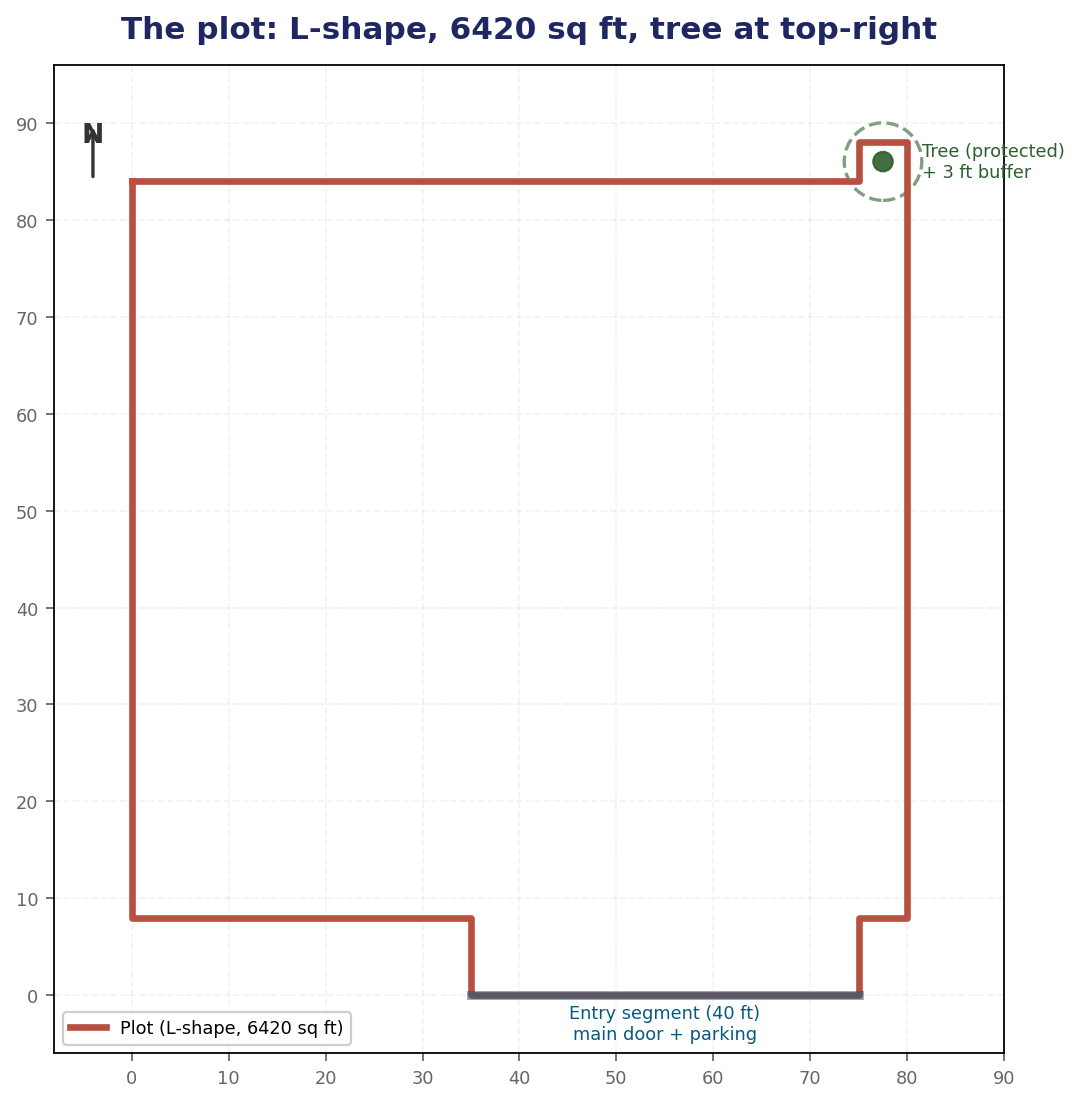
\includegraphics[width=3.0in]{plot_only}}
\caption{The L-shaped residential plot (6{,}420 sq ft) with the protected tree at the top-right and the southern entry segment.}
\label{fig:plot}
\end{figure}

\section{Exterior Stage}
\subsection{Z3 as an optimizer}
The brief's ``maximize area'' is made verifiable by first computing the provably-largest legal footprint. With the four house edges as symbolic reals $x_{\min},x_{\max},y_{\min},y_{\max}$ and plot bounds $[X_0,X_1]\times[Y_0,Y_1]$, the setback constraints are
\begin{equation}
x_{\min}\!\ge\! X_0\!+\!s_{\mathrm{side}},\;\; x_{\max}\!\le\! X_1\!-\!s_{\mathrm{side}},\;\; y_{\min}\!\ge\! Y_0\!+\!s_{\mathrm{front}},\;\; y_{\max}\!\le\! Y_1\!-\!s_{\mathrm{rear}},
\label{eq:setback}
\end{equation}
and because the objective decomposes, Z3 \texttt{Optimize} maximizes width and depth independently:
\begin{equation}
A_{\max}=\big(\max(x_{\max}-x_{\min})\big)\cdot\big(\max(y_{\max}-y_{\min})\big).
\label{eq:maxarea}
\end{equation}
The verifier then enforces a hard \emph{coverage} rule, turning the vague objective into a checkable constraint:
\begin{equation}
A_{\mathrm{house}} \;\ge\; 0.90\,A_{\max}.
\label{eq:coverage}
\end{equation}

\subsection{Generate--verify loop}
The generator (Gemini) emits the four corners and the door as magic comments; the parser extracts them; the Z3 verifier checks nine SBC rules (Eq.~\ref{eq:setback}, the tree buffer, single-side egress, minimum footprint, polygon containment, and Eq.~\ref{eq:coverage}); and on failure an LLM (Llama on Groq) rewrites the violations as actionable feedback. The converged exterior is shown in Fig.~\ref{fig:exterior}.

\begin{figure}[ht]
\centerline{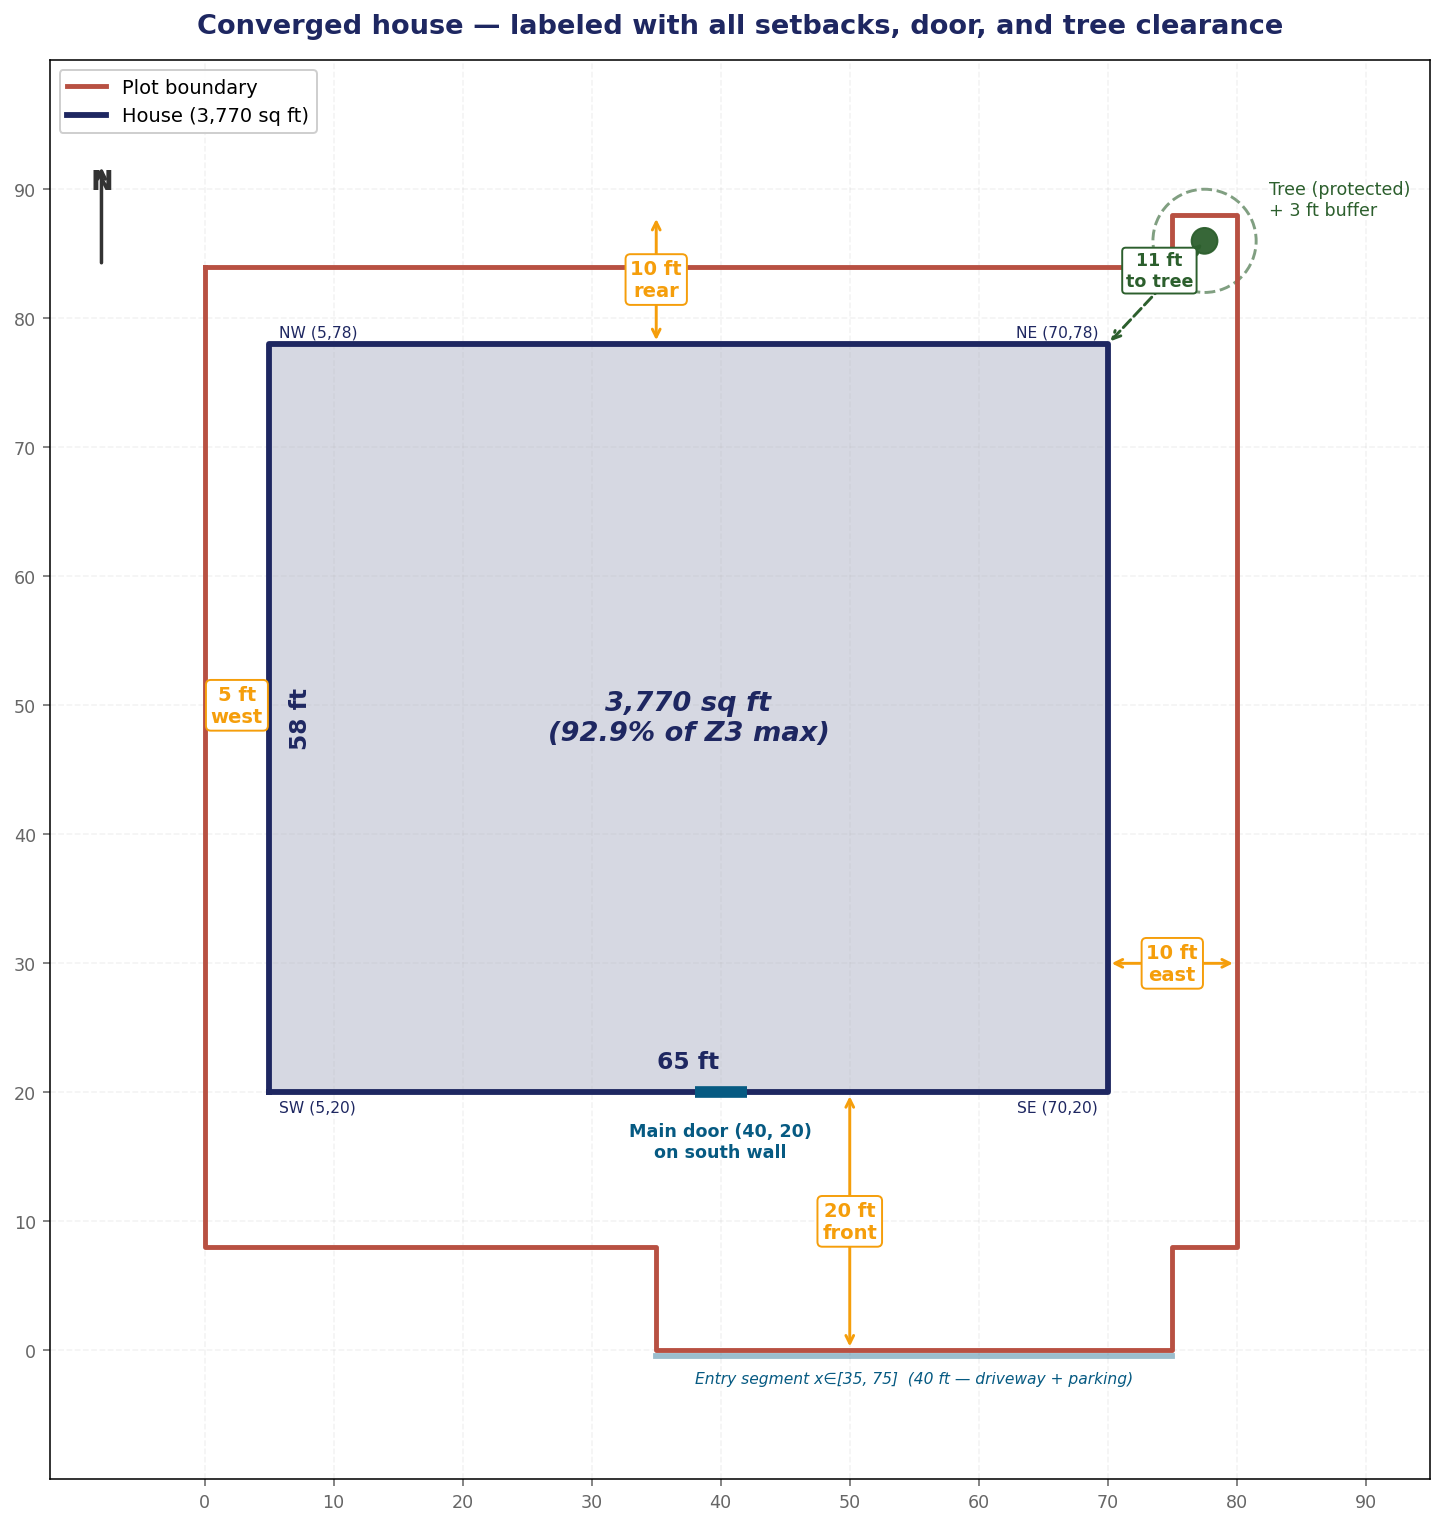
\includegraphics[width=3.2in]{labeled_result}}
\caption{Converged exterior: a verified footprint at 90\% of the Z3-computed maximum, with setbacks, tree clearance and door labelled.}
\label{fig:exterior}
\end{figure}

\section{Interior Stage}
\subsection{Room program and constraints}
The interior must contain the rooms in Table~\ref{tab:program}, sized to IRC minimums. The Z3 interior verifier checks, in addition, non-overlap, exact coverage (within tolerance), the door opening into the living room, bathroom adjacency/sanitation rules, and full connectivity. The complete list is given in Appendix~\ref{app:constraints}.

\begin{table}[!h]
\begin{center}
\begin{tabular}{|l|c|c|c|}
\hline
Room & Count & Min.\ area (sq ft) & Min.\ side (ft) \\
\hline
Living   & 1 & 70 & 7 \\ \hline
Kitchen  & 1 & 70 & 7 \\ \hline
Bedroom  & 3 & 70 & 7 \\ \hline
Bathroom & 2 & 25 & 5 (max 15) \\ \hline
Corridor & $\ge 1$ & --- & 4 (width) \\ \hline
\end{tabular}
\caption{Interior room program and IRC-based minimum sizes.}
\label{tab:program}
\end{center}
\end{table}

\subsection{Three generators}
Three interchangeable generators all target the same verifier:
\begin{enumerate}
\item \textbf{Templates} --- hand-designed, fully-tiled layouts per ``vibe''; instant and always valid; used as the seed and for deterministic quick edits.
\item \textbf{MILP / CBC} --- the cutting-plane solver. Rooms are placed with a big-$M$ disjunctive non-overlap constraint: for every pair $(i,j)$ at least one separation must hold,
\begin{equation}
L_{ij}+R_{ij}+D_{ij}+U_{ij}\ge 1,\qquad L,R,D,U\in\{0,1\},
\label{eq:nonoverlap}
\end{equation}
each binary linked to a linear separation (e.g.\ $x_i+w_i \le x_j + M(1-L_{ij})$). PuLP/CBC solves this by branch-and-cut~\cite{gomory1958cutting}. The MILP interior is shown in Fig.~\ref{fig:milp}.
\item \textbf{LLM (conversational)} --- Gemini/Llama reads a natural-language spatial description (``bedrooms in the three corners, kitchen between the top two''), emits a room list, and Z3 confirms it; on failure the violations are fed back and it retries.
\end{enumerate}
A deterministic \emph{gap-filler} converts any leftover space into thin ($\ge 4$ ft) hallways so the plan tiles to $\approx 100\%$ with no large empty blocks.

\begin{figure}[ht]
\centerline{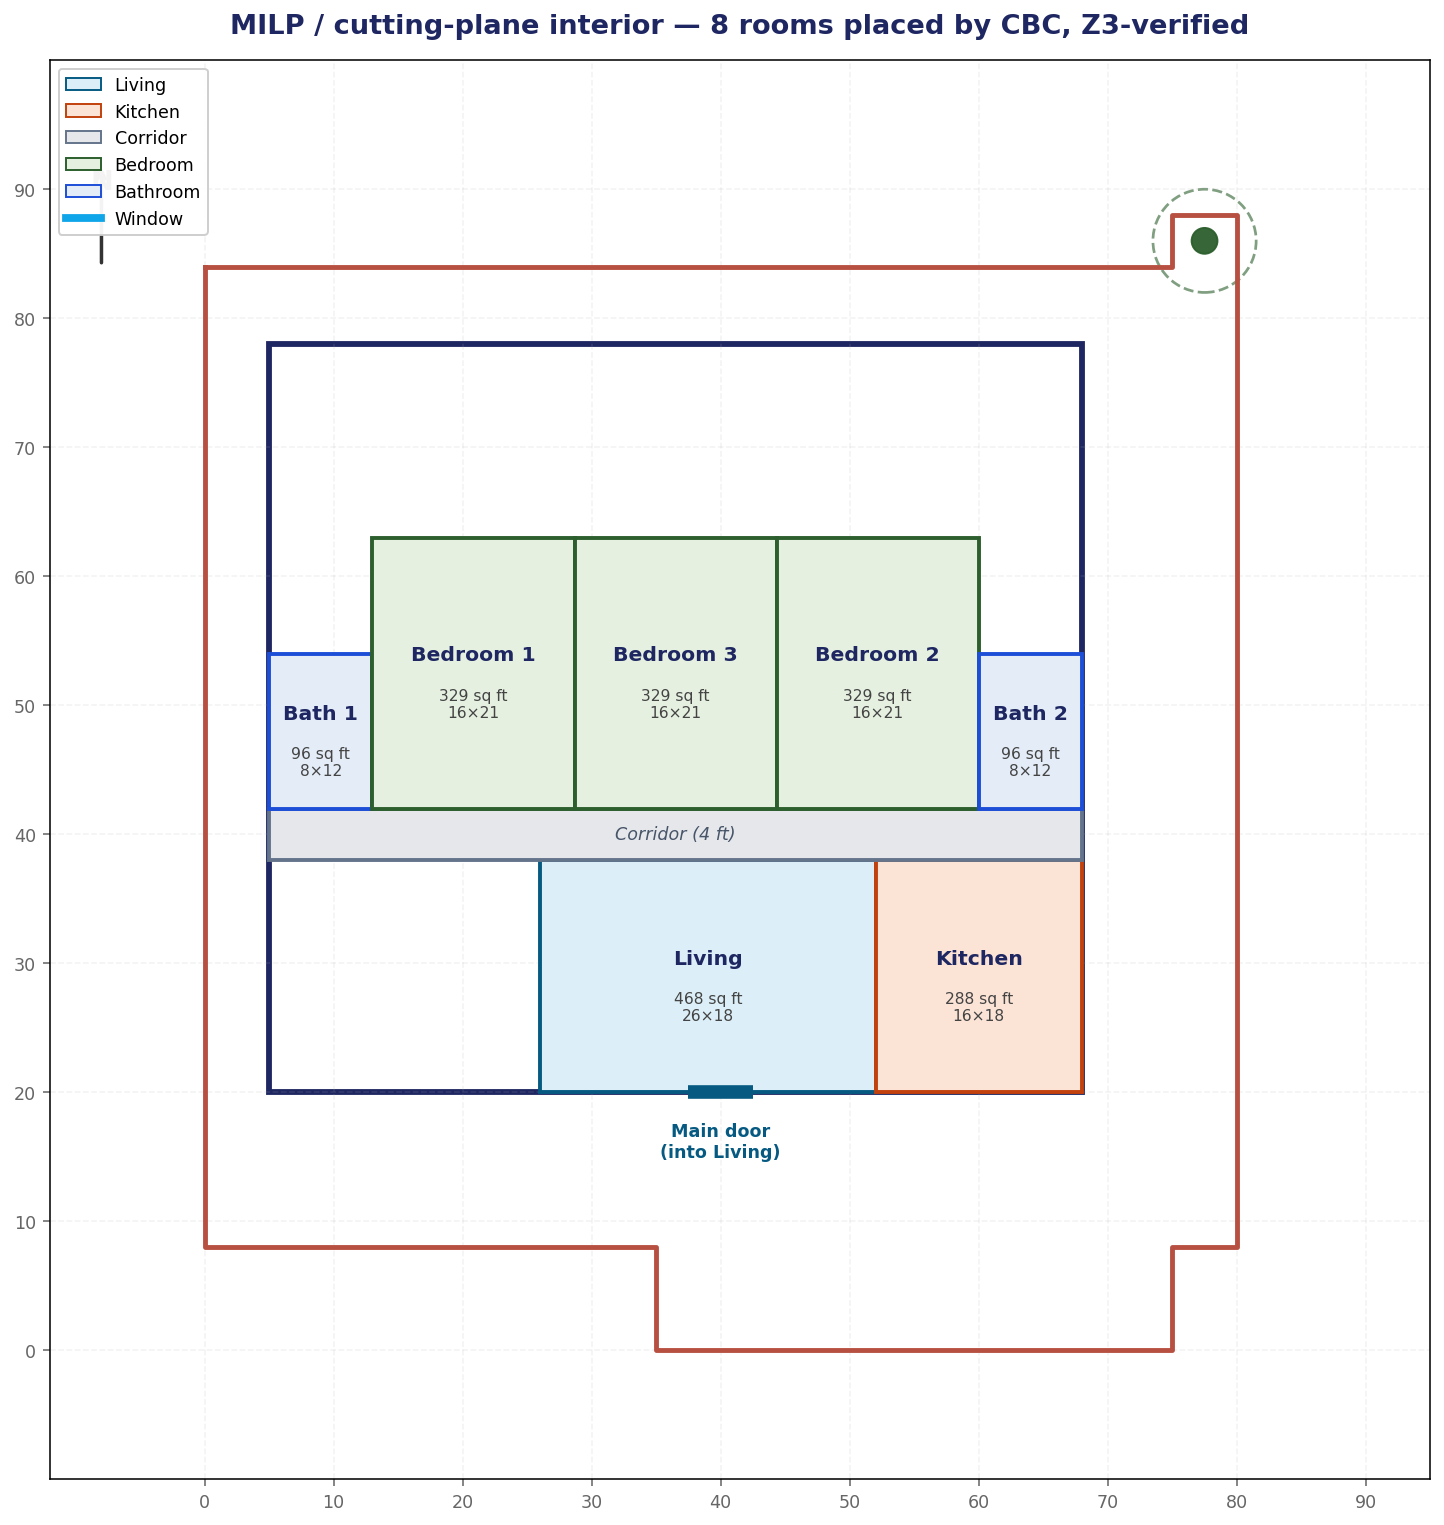
\includegraphics[width=3.0in]{milp_result}}
\caption{Interior generated by the cutting-plane MILP and verified by Z3: eight rooms tiling the footprint with a single corridor band.}
\label{fig:milp}
\end{figure}

\section{Human-in-the-Loop Studio}
The system is delivered as a conversational Streamlit web app~\cite{streamlit}. The user picks a starting ``vibe'', then edits the plan two ways: \emph{quick-change buttons} apply deterministic, always-valid adjustments to the template's cut positions, while \emph{free-text} is handled by the LLM. A layout is shown only if Z3 fully accepts it; otherwise the previous valid plan is kept and the blocking rule is reported. Because correctness lives in Z3, the LLM provider is swappable (Gemini~$\leftrightarrow$~Groq), which proved essential when an API quota was exhausted.

\section{Implementation and System Requirements}
The system is implemented in Python~3.x. Minimum requirements:
\begin{itemize}
\item A modern multi-core CPU --- the MILP and SMT solves run repeatedly inside the interactive loop and benefit from fast single-thread performance.
\item 4--8 GB RAM to hold the solver state and the rendering buffers.
\item Network access for the LLM APIs (Google Gemini, Groq), with the keys stored server-side.
\item Python packages: \texttt{z3-solver}, \texttt{pulp} (with CBC), \texttt{ezdxf}, \texttt{matplotlib}, \texttt{streamlit}, \texttt{google-genai}, \texttt{groq}.
\end{itemize}

% ============================================================ CH 4
\chapter{Results and Discussions}

\section{Exterior Results}
Z3 \texttt{Optimize} proved a maximum legal house of 4{,}060 sq ft. The generate--verify loop converged in two iterations to a footprint at exactly 90\% of that maximum (Table~\ref{tab:ext}, Fig.~\ref{fig:exterior}). The first attempt covered only 57\% of the maximum and was rejected by the coverage rule (Eq.~\ref{eq:coverage}); the feedback agent corrected it on the second pass --- a concrete demonstration of the solver catching and fixing an LLM error.

\begin{table}[!h]
\begin{center}
\begin{tabular}{|l|c|}
\hline
Metric & Value \\
\hline
Plot area & 6{,}420 sq ft \\ \hline
Z3-provable maximum house & 4{,}060 sq ft \\ \hline
Coverage threshold ($\ge 90\%$) & 3{,}654 sq ft \\ \hline
Converged footprint & 3{,}654 sq ft (90\% of max) \\ \hline
Iterations to converge & 2 \\ \hline
\end{tabular}
\caption{Exterior stage results.}
\label{tab:ext}
\end{center}
\end{table}

\section{Interior Results}
The interior generators produce plans that tile the footprint ($\approx 100\%$ coverage) and pass the full Z3 constraint set. Four distinct ``vibe'' templates were designed (Fig.~\ref{fig:vibes}): \emph{Balanced} (even), \emph{Family} (large bedrooms), \emph{Entertainer} (large living), and \emph{Work-from-home} (an oversized study-bedroom). In all four, bedrooms are square-ish (aspect $\le 1.3$) and no two bedrooms share a wall.

\begin{figure}[ht]
\centerline{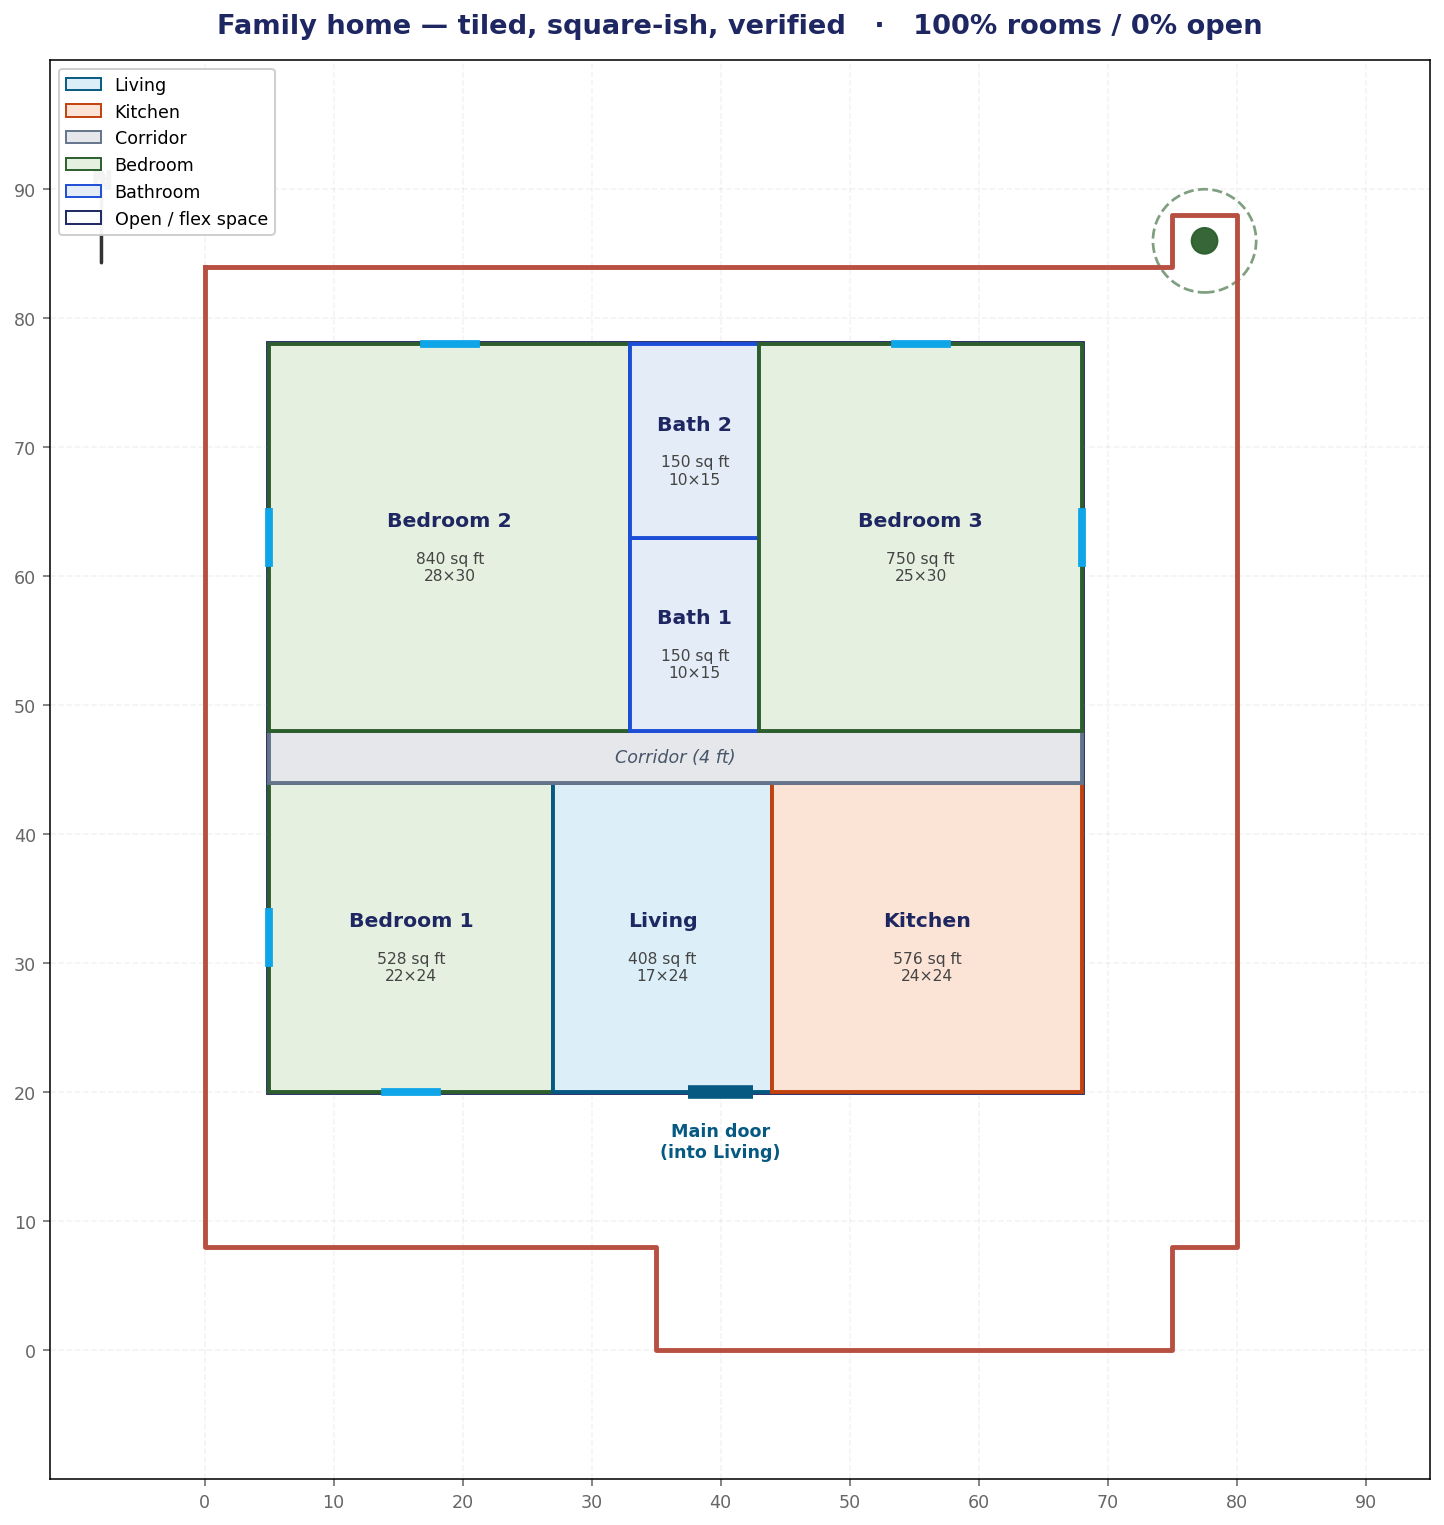
\includegraphics[width=2.5in]{vibe_family}\hspace{0.2in}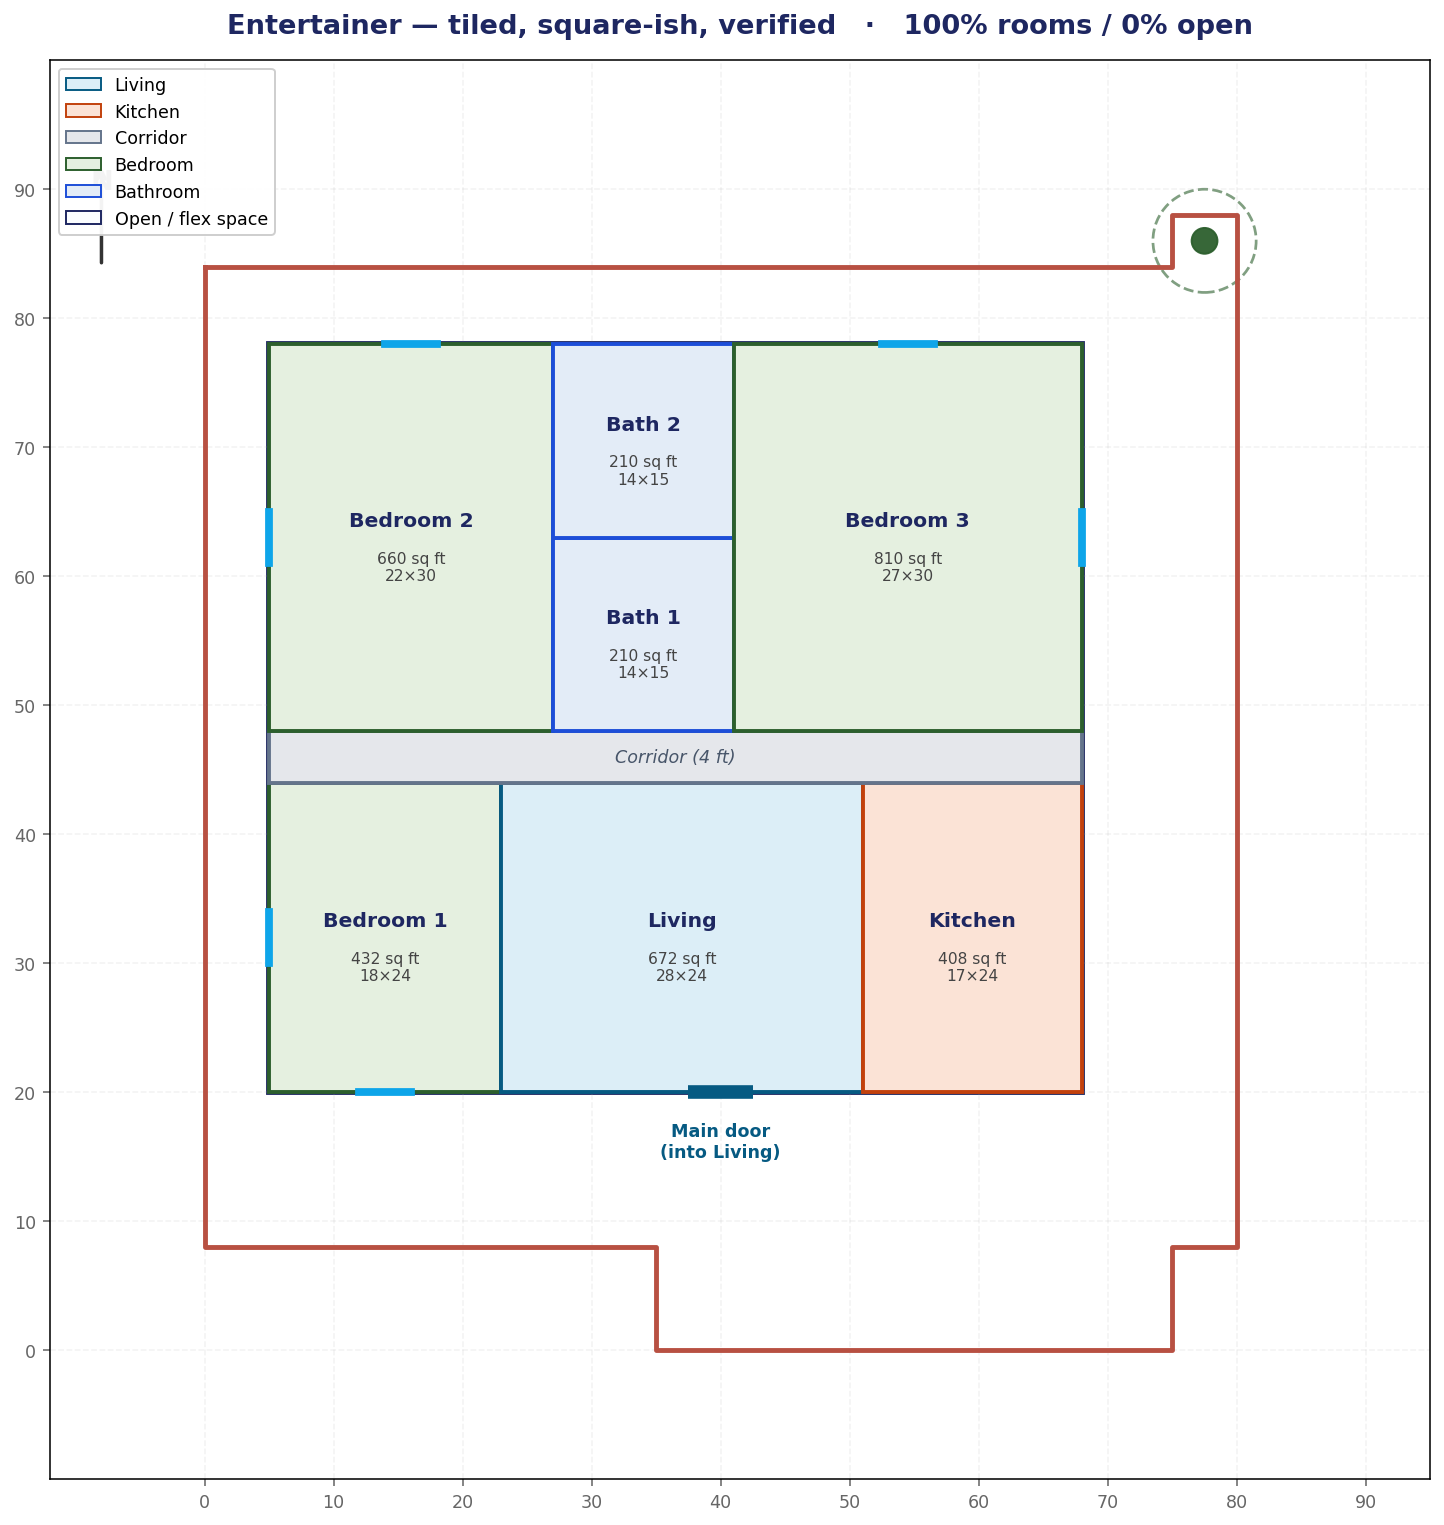
\includegraphics[width=2.5in]{vibe_entertainer}}
\caption{Two of the four verified ``vibe'' layouts: Family (left, large bedrooms) and Entertainer (right, large living room).}
\label{fig:vibes}
\end{figure}

\section{The Conversational Designer}
Given a detailed spatial prompt, the LLM designer places rooms as described, the gap-filler adds halls, and Z3 confirms the result --- typically within two attempts (Fig.~\ref{fig:studio}). This realizes the ``describe it in words, the solver proves it'' interaction.

\begin{figure}[ht]
\centerline{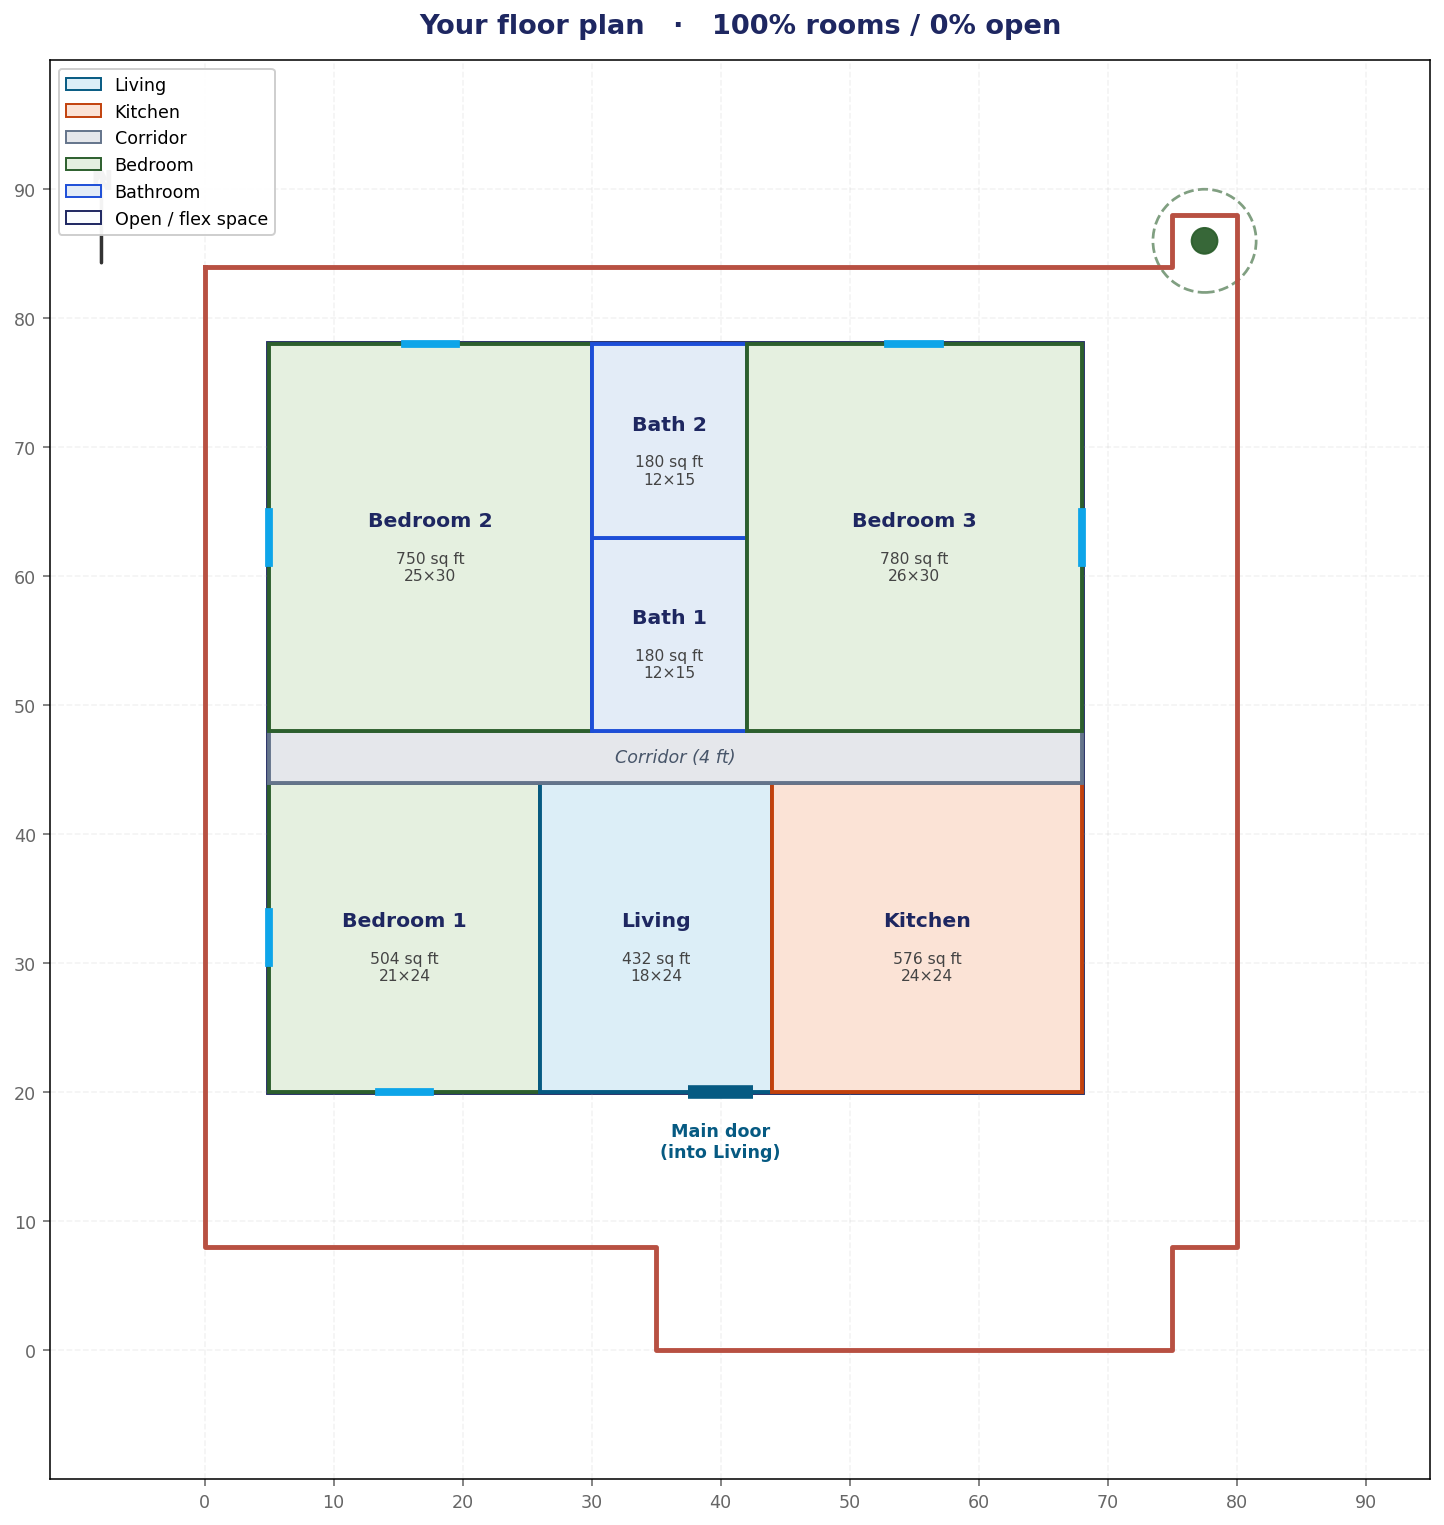
\includegraphics[width=3.0in]{studio_layout}}
\caption{A layout produced from a free-text description and verified by Z3 in the conversational studio.}
\label{fig:studio}
\end{figure}

\section{Engineering Problems Encountered and Fixes}
Most defects surfaced from live testing in the studio. Table~\ref{tab:problems} summarizes them. Figure~\ref{fig:beforeafter} contrasts the worst case --- a large block of wasted space mislabelled as ``corridor'' --- with the fully-tiled fix.

\begin{table}[!h]
\begin{center}
\begin{tabular}{|p{4.3cm}|p{3.8cm}|p{4cm}|}
\hline
Problem observed & Root cause & Fix \\
\hline
Tiny bedrooms, huge living/kitchen & fixed band put all depth into the public zone & tunable sizes + balanced templates \\ \hline
$\sim$35\% left empty as one block & rooms floated; leftover dumped as one rectangle & tiling templates + $\ge 4$ ft halls \\ \hline
Bedrooms too long (16$\times$29) & bedrooms filled the full band depth & square-ish templates ($\le 1.3$) \\ \hline
All four vibes looked identical & same layout, tiny size nudges & four distinct tiled templates \\ \hline
Chat left invalid plans & LLM broke a rule; best invalid shown & commit only if valid (else revert) \\ \hline
Gemini quota (20/day) exhausted & free-tier cap & switched generator to Llama 3.3 (Groq) \\ \hline
\end{tabular}
\caption{Problems encountered during development and their fixes.}
\label{tab:problems}
\end{center}
\end{table}

\begin{figure}[ht]
\centerline{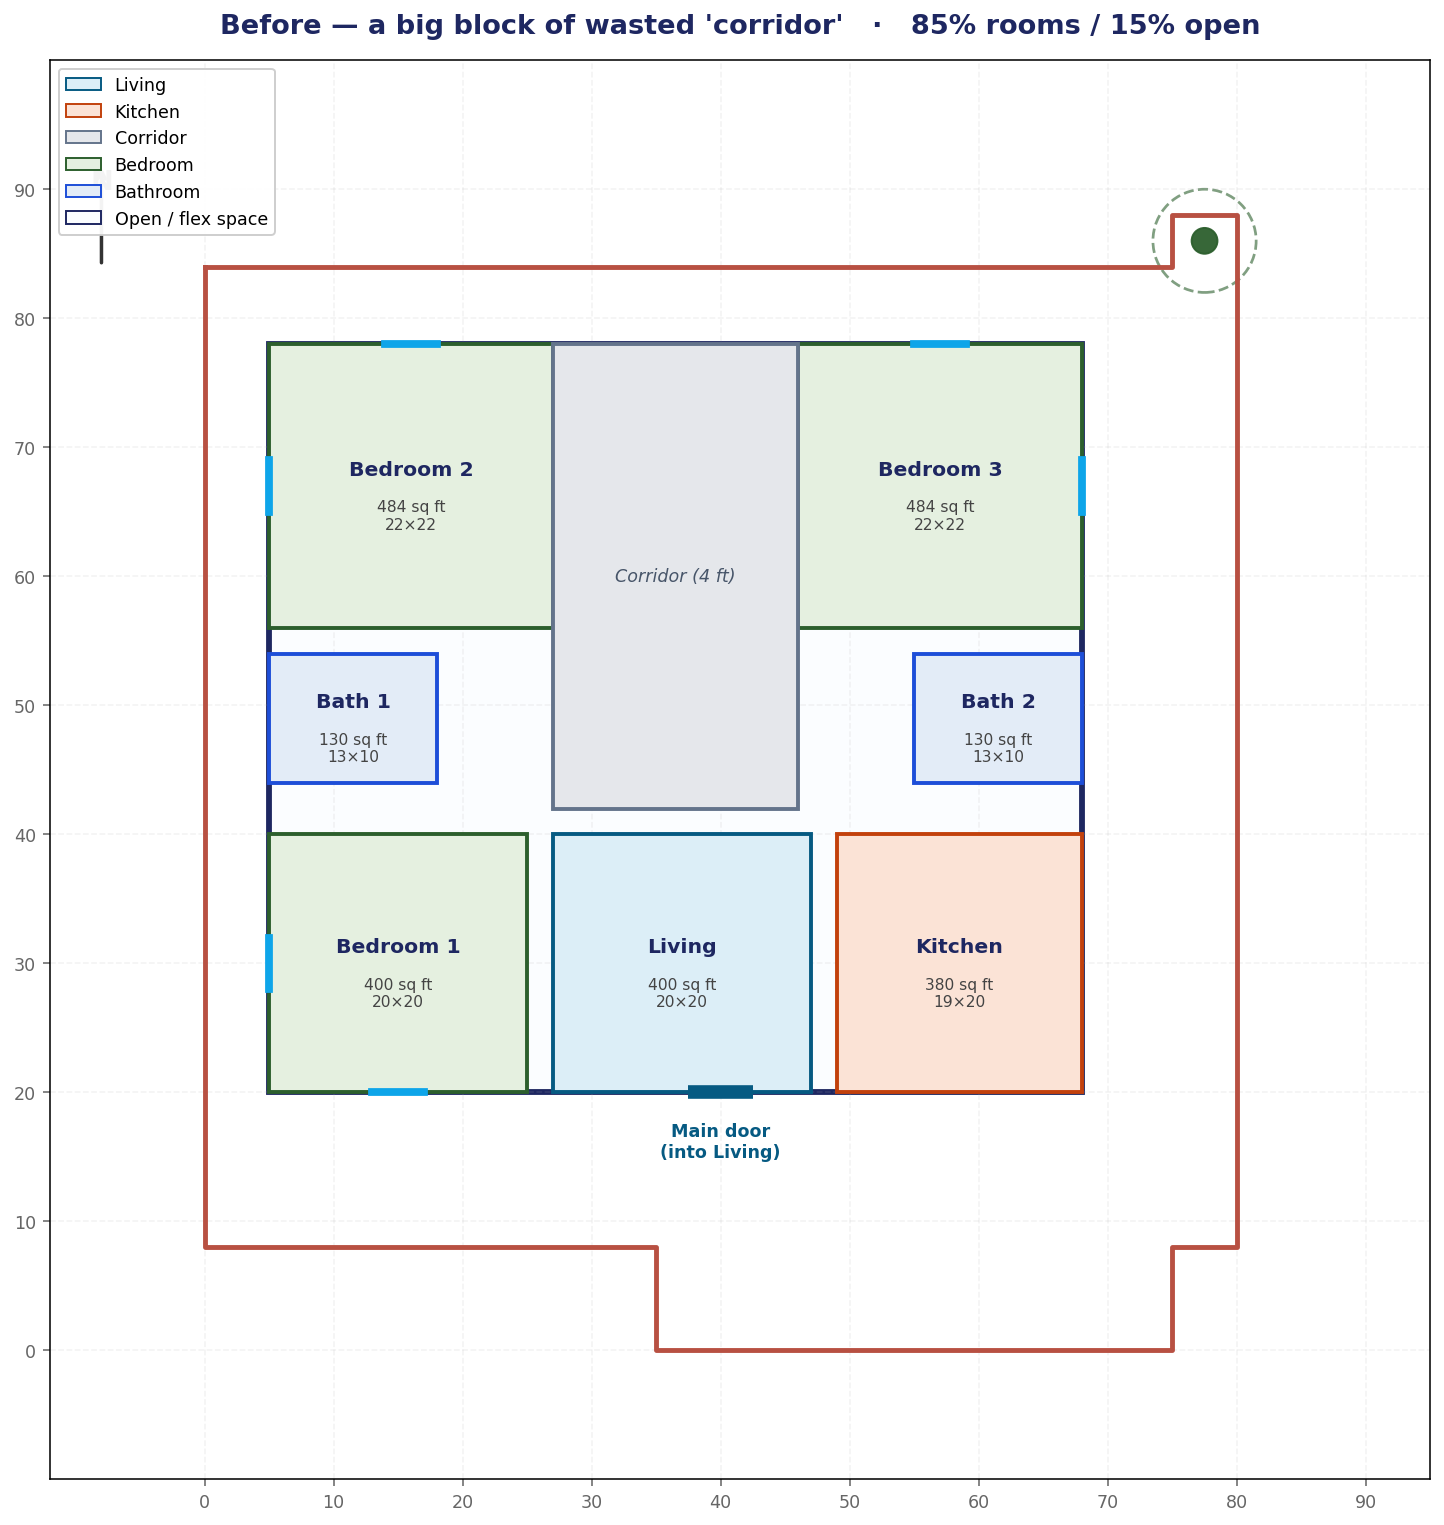
\includegraphics[width=2.5in]{before_block}\hspace{0.2in}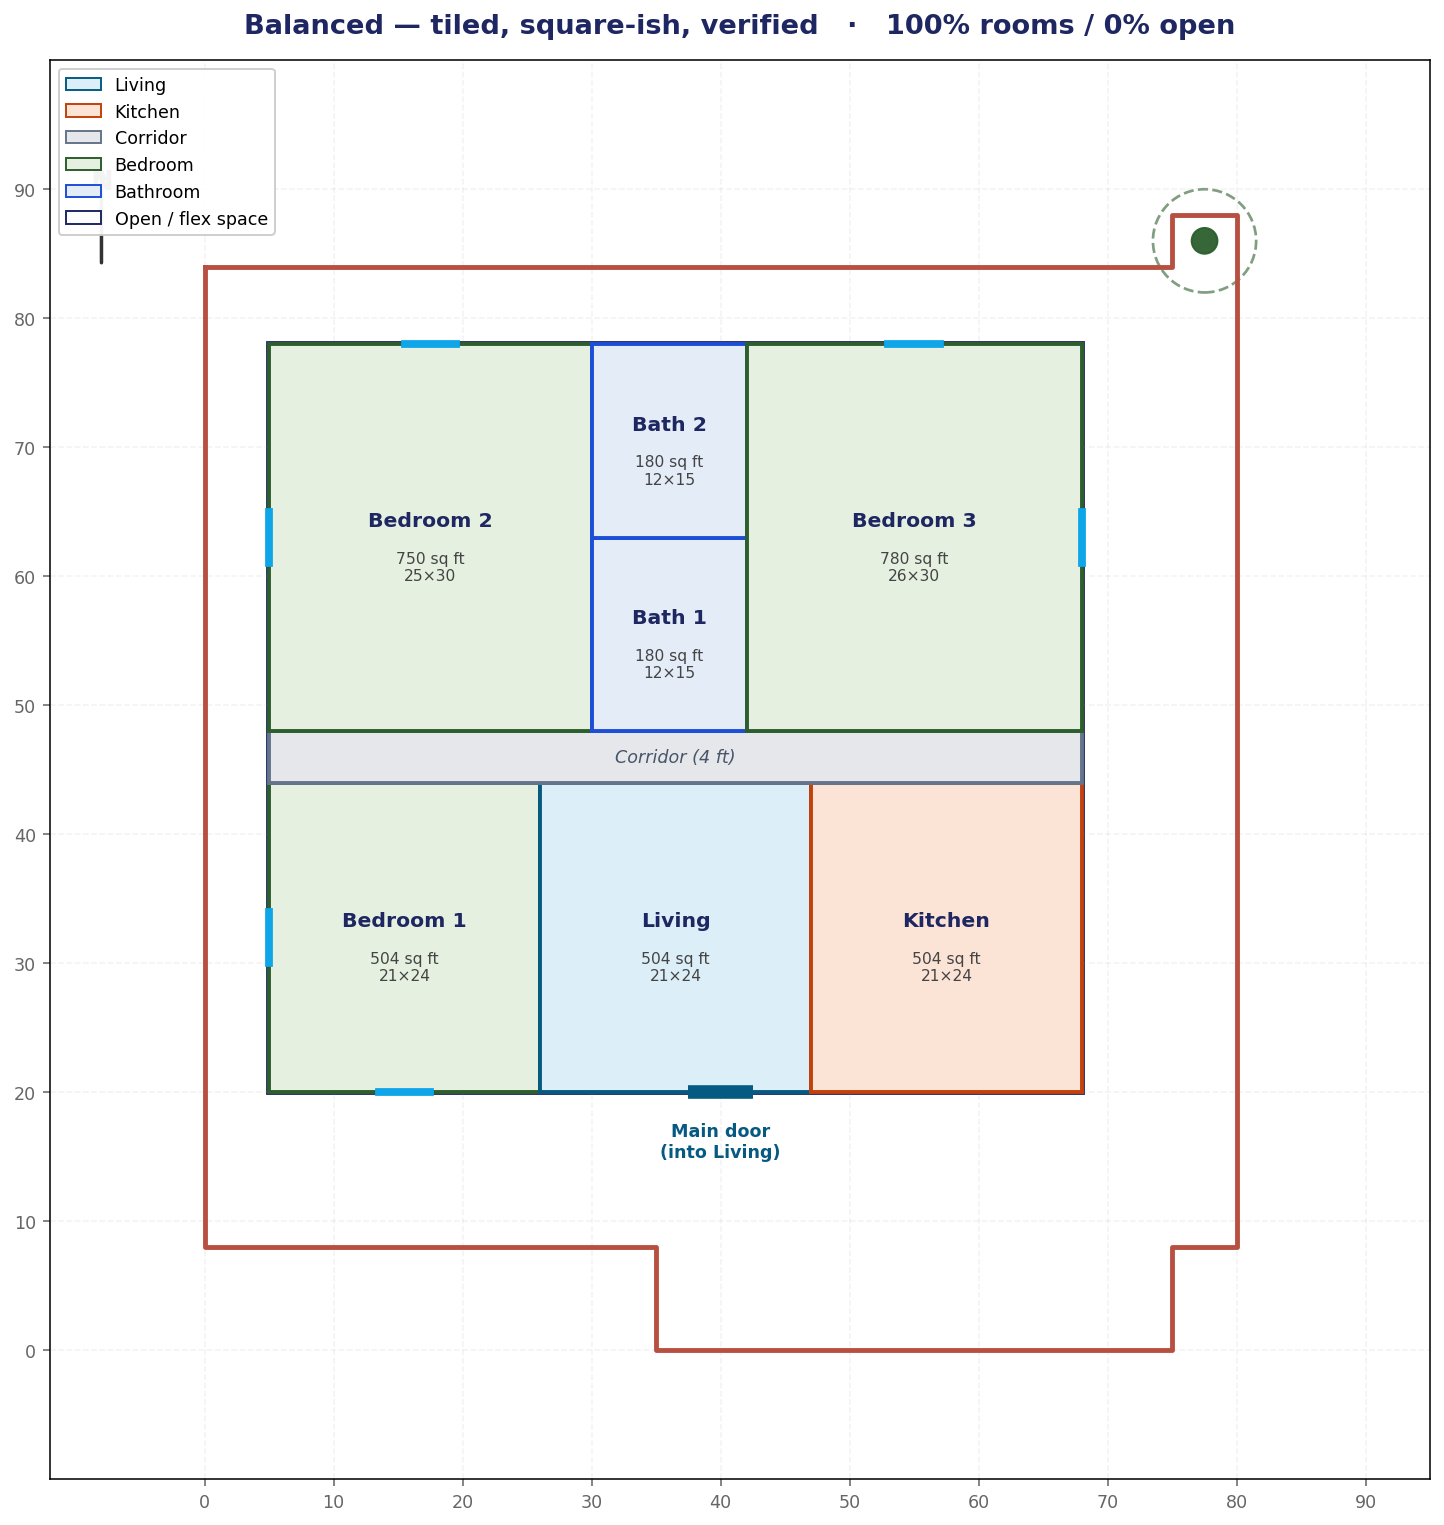
\includegraphics[width=2.5in]{vibe_balanced}}
\caption{Before (left): a large block of wasted ``corridor''. After (right): a fully-tiled, Z3-verified plan with only a thin hallway.}
\label{fig:beforeafter}
\end{figure}

\section{Comparison of Language Models}
Table~\ref{tab:llm} summarizes our experience with the models we ran. The recurring finding across all of them was that LLMs are strong at intent and first-pass generation but unreliable at \emph{constraint-preserving incremental edits}; this is why we route simple edits to a deterministic solver and keep the LLM for descriptions, with Z3 as the always-on judge that makes the generator swappable.

\begin{table}[!h]
\begin{center}
\begin{tabular}{|p{3cm}|p{5cm}|p{5cm}|}
\hline
Model & Strengths & Limitations \\
\hline
Gemini 2.5 Flash & best spatial reasoning; honoured the output format; converged in $\sim$2 iters & 20 requests/day free-tier cap (exhausted mid-work); ``thinking'' hangs (fixed with budget 0) \\ \hline
Llama 3.3 70B (Groq) & very high rate limit, no timeouts; fast; reliable feedback writer & weaker spatial quality as a generator; dropped the output marker prefix \\ \hline
Kimi K2 (Groq) & --- (assigned) & returned 404 \texttt{model\_not\_found}; never ran (availability, not capability) \\ \hline
\end{tabular}
\caption{Comparison of the language models used.}
\label{tab:llm}
\end{center}
\end{table}

% ============================================================ CH 5
\chapter{Conclusions and Future Work}
The project shows that a neuro-symbolic loop --- LLM generation guarded by an SMT verifier --- produces house drawings that are not just plausible but provably code-compliant, and that the same Z3 judge lets us swap generators (LLM, MILP, or templates) freely while preserving correctness. Pairing this with a conversational, human-in-the-loop interface gives a usable tool in which the human sets intent and the solver owns compliance.

\par\noindent Several extensions would improve the results. \emph{Multi-floor} support would stack verified per-floor plans with vertical alignment of stairs and plumbing as new Z3 constraints. A \emph{roof-plan} agent could compute ridges, hips and valleys from the footprint polygon (e.g.\ via the straight skeleton) and verify pitch, drainage and height. \emph{3D diagrams} and \emph{elevations} would follow from extruding the verified plans. On the systems side, a \emph{persistence layer} (project save/load and version history) and an \emph{MCP client--server} decomposition (exposing the Z3 verifier and the drawing tools as services) would turn the prototype into a product, and a \emph{multi-jurisdiction rule pack} would broaden code coverage beyond the current Seattle/IRC subset.

% ============================================================ CH 6
\chapter{Recommendations}
\begin{enumerate}
\item \textbf{Route by task type.} Use a deterministic solver for simple, exact edits and reserve the LLM for genuine natural-language design; this is both more reliable and cheaper.
\item \textbf{Keep Z3 as the single judge.} It makes the generator and the LLM provider replaceable, which directly mitigated the API-quota failure we hit.
\item \textbf{Adopt an MCP architecture.} Expose the verifier, the optimizer and the drawing/export tools as standalone MCP servers so agents (and other apps) can reuse them.
\item \textbf{Harden for production.} Add authentication/authorization, server-side secret management with key rotation, per-user rate limits, hard solver timeouts, and a database with an audit trail of which rules each plan passed.
\item \textbf{Be honest about scope.} Ship a clear disclaimer: the tool verifies an encoded subset of code and is not a substitute for a licensed architect or a permit review.
\end{enumerate}

\bibliography{ref}
\addcontentsline{toc}{chapter}{Bibliography}

% ============================================================ APPENDICES
\begin{appendices}

\chapter{The Interior Constraint Set}
\label{app:constraints}
The Z3 interior verifier checks the following, grouped by purpose:
\begin{itemize}
\item \textbf{Counts:} exactly 3 bedrooms, 2 bathrooms, 1 kitchen, 1 living, and at least one corridor.
\item \textbf{Sizes:} every room meets its IRC minimum area and minimum side; bathrooms are additionally capped at 15 ft per side.
\item \textbf{Structure:} all rooms lie inside the footprint; no two rooms overlap; rooms cover the footprint within tolerance.
\item \textbf{Door / egress:} the front door opens into the living room on the south wall, inset from its side walls.
\item \textbf{Circulation:} a corridor of width $\ge 4$ ft; every room is reachable from every other (connectivity).
\item \textbf{Bathrooms (strict mode):} each bathroom is ensuite to a distinct bedroom and smaller than it; no bathroom abuts the kitchen; the two bathrooms are not adjacent.
\end{itemize}
A \emph{freeform} mode keeps the geometry rules (containment, non-overlap, sizes, door, connectivity, coverage) but relaxes the rigid arrangement rules so that user-described layouts are permitted.

\chapter{The MILP Formulation}
\label{app:milp}
For rooms with fixed sizes $(w_r,h_r)$ and variable lower-left corners $(x_r,y_r)$ inside a footprint of width $W$ and depth $H$, with $M=W+H$:
\begin{align}
& x_r + w_r \le X_1, \quad y_r + h_r \le Y_1 && \text{(containment)} \\
& L_{ij}+R_{ij}+D_{ij}+U_{ij} \ge 1 && \text{(non-overlap, Eq.~\ref{eq:nonoverlap})} \\
& x_i + w_i \le x_j + M(1-L_{ij}) && \text{($i$ left of $j$)} \\
& x_{\mathrm{living}} + \delta \le x_{\mathrm{door}} \le x_{\mathrm{living}} + w_{\mathrm{living}} - \delta && \text{(door in living)}
\end{align}
with analogous big-$M$ links for $R,D,U$. The objective maximizes the smallest bedroom width to balance the bedrooms. PuLP builds the model and CBC solves it by branch-and-cut.

\chapter{Example: Magic Comment and Parsed Layout}
The generator emits a single line that the parser reads without executing any code, e.g.
\begin{verbatim}
# ROOMS: [("Living","living",27,20,47,44),
#         ("Kitchen","kitchen",47,20,68,44), ... ]
\end{verbatim}
A regular expression extracts the bracketed list and \texttt{ast.literal\_eval} converts it to data; the resulting rectangles are then verified by Z3 and rendered to DXF.

\end{appendices}

\end{document}
